\section{Durchführung}
\label{sec:Durchführung}

Der Versuchsaufbau ist in Abbildung \ref{fig:aufbau} dargestellt.
\begin{figure}[H]
  \centering
  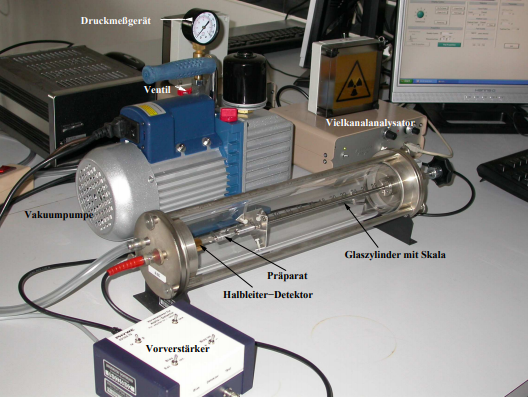
\includegraphics[width=0.8\textwidth]{aufbau.png}
  \caption{Aufbau der Messapparatur\cite{kent}.}
  \label{fig:aufbau}
\end{figure}

Als Strahlungsquelle wird ein Americium-Präparat verwendet, welches sich von außerhalb verschiebbar in 
einem Glaszylinder befindet, der sich mittels einer Vakuumpumpe evakuieren lässt.
Die Alphastrahlung wird mithilfe eines Halbleiter-Sperrschichtzählers detektiert, welcher an
einen Vorverstärker angeschlossen ist, der das Signal an einen Vielkanalanalysator weiterleitet.
Das Signal lässt sich mit einem Programm am Computer analysieren, wenn man ihn mit diesem verbindet.
Hierbei ist darauf zu achten, dass der Schalter im Programm unter \textit{MCA STATUS} auf \textit{connected} gestellt wird.
Da in festen zeitlichen Intervallen gemessen wird, muss der Zählmodus auf \textit{AUTO} gestellt und als Bedingung
\textit{Measurement time} ausgewählt werden. Anschließend wird das jeweilige Messintervall eingetragen.

Um das Grundrauschen bei der Messung zu unterdrücken, muss vor Beginn der Messung
am Vielkanalanalysator eine Diskriminatorschwelle eingestellt werden. Hierfür wird
die Strahlungsquelle bei Umgebungsdruck möglichst weit vom Detektor entfernt und
die Diskriminatorschwelle so eingestellt, dass keine Pulse mehr gezählt werden.
Danach wird die Strahlungsquelle so nah an den Detektor herangebracht, dass der Computer
wieder beginnt Pulse zu zählen. Anschließend wird die Röhre evakuiert und die Messung beginnt.

In Intervallen von $50\,\si{\milli\bar}$ werden die Gesamtanzahl der Pulse in einem Zeitintervall
von $120\,\si{\second}$ und der Kanal, in dem das Maximum der Pulse liegt, notiert.

Zur Überprüfung der Statistik des radioaktiven Zerfalls wird in einem Intervall
von $10\,\si{\second}$ die Anzahl der registrierten Pulse in der evakuierten Röhre notiert. Diese
Messung wird 100 mal wiederholt.